
First suggested in \cite{Granade:2012kj} and since developed \cite{wiebe2014qhlpra, Wiebe:2014qhl} 
    and implemented \cite{gentile2020learning, wang2017experimental}, 
\gls{qhl} is a machine learning algorithm for the optimisation of a given \gls{hamiltonian} parameterisation 
    against a quantum system whose model is known a priori. 
Given a target quantum system, \gls{q}, known to be described by some \gls{hamiltonian} $\hat{H}(\vec{\alpha})$, 
    \gls{qhl} optimises $\vec{\alpha}$.
This is achieved by interrogating \gls{q} and comparing its outputs against proposals $\vec{\alpha}_p$. 
In particular, an \gls{experiment} is designed, consisting of an input state, $\ket{\psi}$, and an evolution time, $t$.
This \gls{experiment} is performed on \gls{q}, whereupon its measurement yields the datum $d \in \{0, 1\}$ -- 
    i.e. the eigenstate $\ket{d} \in \{ \ket{0}, \ket{1}\}$ is observed -- 
    according to the expectation value $\lvert \bra{\psi} e^{-i \ho t} \ket{\psi} \rvert^2$. 
Then, on a trusted (quantum) simulator, proposed parameters $\vec{\alpha}_p$ are encoded to the 
    known Hamiltonian, and the same \gls{probe} state is evolved for the chosen $t$ and projected on to $\ket{d}$, 
    i.e. $\lvert \bra{d} e^{-i \hat{H}(\vec{\alpha}_p) t } \ket{\psi} \rvert^2 $ is computed.
The task for \gls{qhl} is then to find $\vec{\alpha}^{\prime}$ for which this quantity 
    is close to 1 for all values of $(\ket{\psi}, t)$, 
    i.e. the parameters input to the simulation produce dynamics consistent with those measured from \gls{q}.
\par 

The procedure is as follows. 
A \emph{prior} probability distribution $\pra$ in a parameter space of dimension $\lvert \al \rvert$ 
    is initialised to represent the constituent parameters of $\al$. 
$\pra$ is typically a multivariate normal (Gaussian) distribution; 
    it is therefore necessary to pre-suppose some mean and width for each parameter in $\al$. 
This imposes prior knowledge on the algorithm whereby the programmer must decide the range in 
    which parameters are \emph{likely} to fit:
    although \gls{qhl} is generally robust and capable of finding parameters outside of this prior,
    the prior must at least capture the order of magnitude of the target parameters. 
It is important to understand, then, that \gls{qhl} removes the prior knowledge 
    of precisely the parameter representing an interaction in \gls{q}, but does rely on a ball-park estimate thereof from which to start. 
\par 

In short, \gls{qhl} samples parameter vectors $\al_p$ from $\pra$, 
    simulates \glspl{experiment} by computing the \emph{likelihood} $\lvert \bra{d} e^{-i \hat{H}(\al_p)t} \ket{\psi} \rvert^2$
    for \glspl{experiment} ($\ket{\psi}, t)$ designed by a \gls{qhl} heuristic subroutine, 
    and iteratively improves the probability distribution of the parameterisation $\pra$ 
    through standard \emph{Bayesian inference}. 
A given set of $(\ket{\psi}, t)$ is called an \emph{experiment}, since it corresponds to preparing, evolving and measuring \gls{q} 
once\footnote{Experimentally, this may involve repeating a measurement many times to determine a majority result and to mitigate noise.}. 
\gls{qhl} iterates for \gls{nexp} \glspl{experiment}. 
The parameter vectors sampled are called \emph{\glspl{particle}}: there are \gls{nprt} \glspl{particle} used per experiment. 
Each \gls{particle} used incurs one further calculation of the \gls{likelihood} function -- 
    this calculation, on a classical computer, is exponential in the number of qubits of the model under consideration
    (because each unitary evolution relies on the exponential of the $2^n \times 2^n$ \gls{hamiltonian} matrix of $n$ qubits). 
Likewise, each additional \gls{experiment} incurs the cost of calculation of \gls{nprt} \glspl{particle}, 
    so the total cost of running \gls{qhl} to train a model is $\propto \Ne \Np$.
It is therefore preferable to use as few \glspl{particle} and \glspl{experiment} as possible, 
    though it is important to include sufficient resources that the parameter estimates have the opportunity to converge. 
Access to a fully operational, trusted quantum simulator admits an exponential 
    speedup by simulating the unitary evolution instead of computing the matrix exponential classically.
\par 

\section{Bayes' rule}
Bayes' rule is used to update a probability distribution describing hypotheses, $\Pr(\textrm{hypothesis})$, when presented with new information (data).
That is, the probabilty that a hypothesis is true is replaced
    by the initial probability that is was true, $\Pr(\textrm{hypothesis})$, multiplied by 
    the  \gls{likelihood} that the new data would be observed were that hypothesis true, 
    $\Pr(\textrm{data} | \textrm{hypothesis})$, 
    normalsied by the probability of observing that data in the first place, $\Pr(\textrm{data})$. 
It is stated as
    \begin{equation}\label{eqn:bayes_rule}
        \Pr( \textrm{hypothesis} | \textrm{data} ) = 
        \frac{ \Pr( \textrm{data} | \textrm{hypothesis} ) \times \Pr( \textrm{hypothesis} )}{ \Pr(\textrm{data})}.
    \end{equation}
\par 
We wish to represent our knowledge of \gls{hamiltonian} parameters with a distribution, $\Pr(\al)$:
    in this case hypotheses $\al$ attempt to describe data, $\expdata$, measured from the target quantum system,  
    from a set of \glspl{experiment} $\expset$, so we can rewrite Bayes' rule as 
\begin{equation}\label{eqn:qhl_bayes_rule}
    \Pr(\vec{\alpha} | \expdata; \expset) = \frac{\Pr(\expdata| \vec{\alpha}; \expset) \ \Pr(\vec{\alpha})}{\Pr(\expdata|\expset)}.
\end{equation}

We can consider \cref{eqn:qhl_bayes_rule} at the level of single \emph{\glspl{particle}} (individual vectors in the parameter space), 
    sampled from $\Pr(\al)$:
    \begin{equation}\label{eqn:particle_bayes_rule}
        \Pr(\al_p | d; e) = \frac{ \Pr(d | \ \al_p; \ e ) \ \Pr(\al_p) } {\Pr(d | e)}
    \end{equation}

where 
\begin{easylist}[itemize]
    & $e$ are the experimental controls of a single \gls{experiment}, e.g. evolution time and input \gls{probe} state;
    & $d$ is the datum, i.e. the (usually) binary outcome of measuring \gls{q} under conditions $e$;  
    & $\al_p$ is the \emph{hypothesis}, i.e. a single parameter vector, called a particle, sampled from $\Pr(\al)$;
    & $\Pr(\al_p | d; e)$ is the \emph{updated} probability of this \gls{particle} following the \gls{experiment} $e$, 
        i.e. accounting for new datum $d$, the probability that $\al=\al_0$;
    & $\Pr(d |\al_p ; e)$ is the \gls{likelihood} function, 
        i.e how likely it is to have measured the datum $d$ from the system assuming $\al_p$ are the true parameters
        and the \gls{experiment} $e$ was performed; 
    & $\Pr(\al_p)$ is the probability that $\al_p=\al_0$ according to the prior distribution $\Pr(\al)$, 
        which we can immediately access; 
    & $\Pr(d|e)$ is a normalisation factor, the chance of observing $d$ from \gls{experiment} $e$ irrespective of the underlying hypothesism 
        such that $\sum_{\{d\}} \Pr(d|e) = 1$.
\end{easylist}

In order to compute the updated probability for a given particle, then, all that is required is a value for the \gls{likelihood} function.
This is equivalent to the expectation value of projecting $\ket{\psi}$ onto $\ket{d}$, after evolving $\hat{H}(\al_p)$ for $t$, i.e. 
\begin{equation}
    \label{eqn:likelihood}
    \Pr(d | \al; e) = \lvert \bra{d} e^{-i \hat{H}(\al_p)t} \ket{\psi} \rvert^2,   
\end{equation}
    which can be simulated clasically or using a quantum simulator (see \cref{sec:likelihood}). 
It is necessary first to know the datum $d$ (either 0 or 1) which was projected by \gls{q} under experimental conditions. 
Therefore we first perform the \gls{experiment} $e$ on \gls{q} 
    (preparing the state $\ket{\psi}$ evolving for $t$ and projecting again onto $\bra{\psi}$)
    to retrieve the datum $d$. 
$d$ is then used for the calculation of the \gls{likelihood} for each \gls{particle} sampled from $Pr({\al})$. 
Each particle's probability can be updated by \cref{eqn:particle_bayes_rule}, 
    allowing us to redraw the entire probability distribution.
We can hence compute a \emph{posterior} probability distribution
    by performing this routine on a set of \gls{nprt} \glspl{particle}:
    we hypothesise \gls{nprt} parameterisations $\al_i$ sampled from $\Pr(\al)$, 
    and update their $\Pr(\al_i)$ in proportion to their likelihood.
In effect, hypotheses (\glspl{particle}) which are found to be highly likely are given increased credence, 
    while those with low likelihood have their credence decreased. 

\section{Sequential Monte Carlo}\label{sec:smc}
\begin{figure}
    \setcounter{subfigure}{0}

    \centering
    \subfloat{
        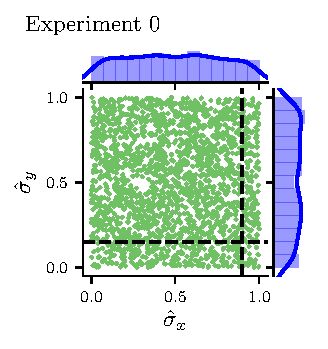
\includegraphics{algorithms/figures/smc_demo/epoch_0.pdf}
    }
    \subfloat{
        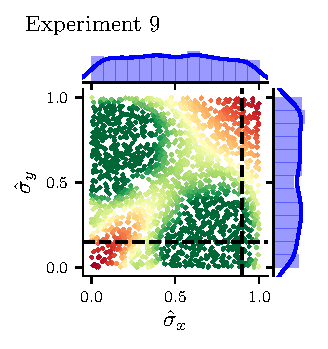
\includegraphics{algorithms/figures/smc_demo/epoch_9.pdf}
    }
    \subfloat{
        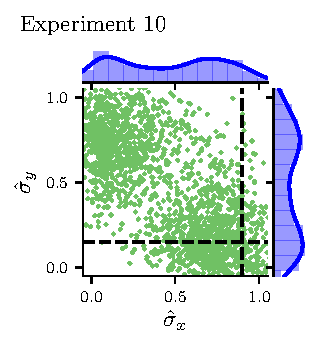
\includegraphics{algorithms/figures/smc_demo/epoch_10.pdf}
    }
    % \hspace{0mm}
    
    \subfloat{
        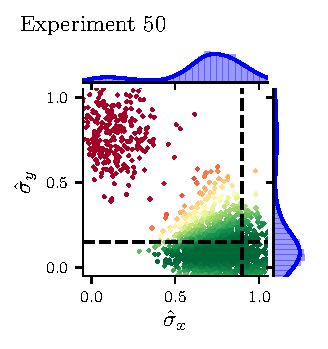
\includegraphics{algorithms/figures/smc_demo/epoch_50.pdf}
    }
    \subfloat{ 
    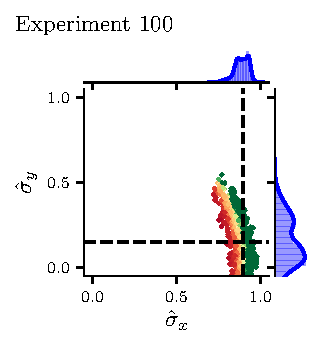
\includegraphics{algorithms/figures/smc_demo/epoch_100.pdf}
    }
    \subfloat{ 
    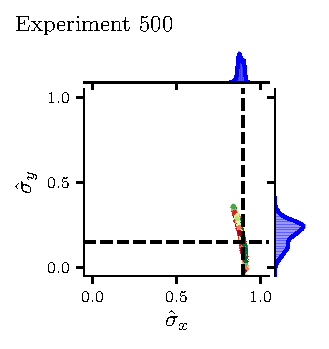
\includegraphics{algorithms/figures/smc_demo/epoch_500.pdf}
    }
    % \hspace{0mm}
    \subfloat{
        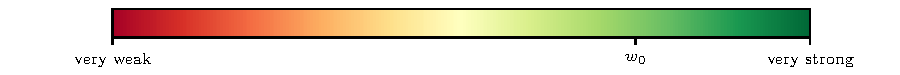
\includegraphics{algorithms/figures/smc_demo/cbar.pdf}
    }
    \caption[Quantum Hamiltonian learning via sequential Monte Carlo]{
        \Acrfull{qhl} via \gls{smc}. 
        The studied model has two terms, $\{\sx, \sy\}$ with true parameters $\alpha_{x}=0.9, \alpha_y=0.15$ (dahsed lines), 
            with resources $\Ne=500, \Np=2000$ for training the model. 
        Crosses represent \glspl{particle}, while the distribution $\Pr(\alpha_p)$ for each 
            parameter can be seen along the top and right-hand-sides of each subplot. 
        Both parameters are assigned a uniform probability distribution $\mathcal{U}(0,1)$, representing our prior knowledge of the system. 
        \textbf{a,} \gls{smc} samples \gls{nprt} \glspl{particle} from the initial joint probability distribution, 
            with \glspl{particle} uniformly spread across the unit square, each assigned the starting \emph{weight} $w_0$. 
            At each \gls{experiment} $e$, each of these \glspl{particle}' \gls{likelihood} is computed according to \cref{eqn:particle_bayes_rule}
            and its weight is updated by \cref{eqn:qhl_weights}.
        \textbf{b,} after 9 \glspl{experiment}, the weights of the sampled \glspl{particle} are sufficiently informative that we know we can 
            discard some \glspl{particle} while most likely retaining the true parameters. 
        \textbf{c,} \gls{smc} resamples according the current $\Pr(\al)$, 
            i.e. having accounted for the \glspl{experiment} and \glspl{likelihood}  observed to date, 
            a new batch of \gls{nprt} \glspl{particle} are drawn, and each reassigned weight $w_0$, 
            irrespective of their weight prior to resampling.  
        \textbf{d-e,} Afer further \glspl{experiment} and resamplings, \gls{smc} narrows $\Pr(\al)$ to a region around the true parameters. 
        \textbf{f,} The final \emph{posterior} distribution consists of two narrow distributions centred on $\alpha_x$ and $\alpha_y$. 
        By taking the mean of the posterior distribution, we approximate the parameters of interest as $\al^{\prime}$. 
    }
    \label{fig:qhl_smc}
\end{figure}
\glsreset{smc}
In practice, \gls{qhl} samples from and updates $\Pr(\al)$  via \gls{smc}.
\gls{smc} samples the \gls{nprt} \glspl{particle} from $\Pr(\al)$, and assigns each \gls{particle} a weight, $w_0 = 1/\Np$.
Each \gls{particle} corresponds to a unique position in the parameters' space, i.e. $\al_p$.
Following the calculation of the likelihood, $\Pr(d | \al_p; e)$, 
    the weight of \gls{particle} $p$ is updated from its initial value of $w_p^{\textrm{old}}$ by \cref{eqn:qhl_weights}.
\begin{equation}\label{eqn:qhl_weights}
    w_p^{\textrm{new}} = \frac{\Pr(d | \al_p; e) \times w_p^{\textrm{old}} } { \sum\limits_{p} w_p \Pr(\al_p | d; e) }
\end{equation}

In this way, strong \glspl{particle} -- with high $\Pr(d | \al_p; e)$ -- have their weight increased, 
    while weak \glspl{particle} (low $\Pr(d | \al_p; e)$) have their weights decreased, 
    and the sum of weights remains normalised. 
Within a single experiment, the weights of all \gls{nprt} \glspl{particle} are updated:
    we \emph{simulataneously} update sampled \glspl{particle}' weights as well as $\Pr(\al)$. 
The procedure of updating \glspl{particle}' weights iterates for the subsequent experiment, using the \emph{same} \glspl{particle}: 
    we do \emph{not} redraw \gls{nprt} \glspl{particle} for every experiment.
Eventually, the weights of most \glspl{particle} fall below a threshold, $r_t$, 
    meaning that only that fraction of \glspl{particle} have reasonable \gls{likelihood} of being $\al_0$.
At this stage, \gls{smc} \emph{resamples}, i.e. selects new \glspl{particle}, according to the updated $\Pr(\al)$\footnotemark.
Then, the new \glspl{particle} are in the range of parameters which is known to be more likely, 
    while \glspl{particle} in the region of low-weight are effectively discarded. 
Usually, we set $r_t=0.5$, although this \gls{hyperparameter} can have a large impact 
    on the rate of learning, so can be optimised in particular circumstances, 
    see \cref{fig:param_learning_vary_particles}.
\par 
This procedure is easiest understood through the example presented in \cref{fig:qhl_smc}, 
    where a two-parameter \gls{hamiltonian} is learned starting from a uniform distribution. 
$\Np=2000$ \glspl{particle} are used to propose hypotheses distributed evenly throughout the parameter space, 
    each of which are subject to weight updates as outined above. 
In this example, after 9 \glspl{experiment} the \glspl{particle} around the diagonal ($x=y$) are deemed unlikely, 
    while clusters form in the opposite corners where the algorithm finds the hypotheses credible. 
Before the tenth experiment, the algorithm resamples, i.e. reassigns weights based on the present $\Pr(\al)$. 
The algorithm iteratively reassigns weight to \glspl{particle} based on their likelihoods, redraws $\Pr(\al)$ and resamples. 
We show the state of the \glspl{particle} after 50, 100 and 500 \glspl{experiment},
    with the overall result of a highly peaked parameter distribution, 
    whose centre is near the target parameters. 

\footnotetext{
    \Glspl{particle} are \emph{resampled} according to a resampling algorithm. 
    Throughout this thesis, we always use the Liu-West resampling algorithm \cite{liu2001combined}.
}

\section{Likelihood}\label{sec:likelihood}
The fundamental step within \gls{qhl} is the calculation of  \gls{likelihood}, 
    which enables updates of the probability distribution in \cref{eqn:particle_bayes_rule}. 
The key to the learning algorithm is that \gls{likelihood} can be retrieved from the Born rule, 
    which captures how likely a given a quantum system is to be measured in an eigenstate.
When we have retrieved a datum, $d$, from \gls{q}, we can compute the probability that \gls{q} 
    would be measured in the corresponding eigenstate $\ket{d}$ -- this probability serves as the likelihood, 
    and is given by \cref{eqn:likelihood}.
\par 

In some cases, it is feasible to derive the closed form of the \gls{likelihood}, 
    for example as a simple expression in terms of the \gls{hamiltonian} parameters, 
    which we will exemplify in \cref{sec:analytical_likelihood}. 
Closed form likelihoods allow for rapidly testing hypothetical parameters for comparison against 
    the observed data, so \gls{qhl} can feasibly be run with high \gls{nexp}, \gls{nprt}.  
In general, however, it is not possible to derive the closed form of the likelihood, 
    and instead the \gls{likelihood} must be computed through \cref{eqn:likelihood}, 
    which can be done either on a classical or quantum simulator. 
The case where the \gls{likelihood} is computed on a quantum simulator is referred to as \gls{qle}
    \cite{Wiebe:2014qhl, wang2017experimental},
    and can leverage any algorithm for the calculation of \gls{hamiltonian} dynamics to achieve \emph{quantum speedup}
    \cite{berry2015hamiltonian, childs2018toward}. %TODO references for \gls{hamiltonian} dynamics
\par 
In this thesis, we do not implement the presented algorithms on quantum hardware,
    instead investigating their performance using idealised classical simulations, i.e. \gls{cle}. 
The reliance on classical resources demands that \cref{eqn:likelihood} be computed explicitly, 
    notably involving the matrix exponential $e^{-i\hat{H}(\al_p) t}$.
Since the \gls{hamiltonian} matrix scales with the size of the simulated system,
    running \gls{qhl} for an $n$-qubit systems requires exponentiation of its $2^n \times 2^n$ \gls{hamiltonian} matrix, 
    in order to compute the exact likelihoods required for learning. 
This overhead restricts the applicability of \gls{cle}: 
    $n=11$-qubit systems' \glspl{hamiltonian} exhaust the memory capacity of most conventional classical computers.
In practice, \gls{qhl} is limited by the computation of the total $\Ne\Np$ matrix exponentials required for training:
    we will only entertain systems which can be represented by \glspl{hamiltonian} of up to $n=8$ qubits. 
In principle, larger systems could be condensed for simulation on available classical resources, 
    or those resources used more efficiently \cite{rudi2020approximating}, 
    but the remit of this thesis can be fulfilled with demonstrations in the domain $n\leq8$ qubits, 
    so we do not endeavour to find the most effective classical strategies.
\par 

Adopting the notation used by QInfer \cite{qinfer-1_0}, upon which our software builds, 
    the expectation value for a the unitary operator is given by
\begin{equation}\label{eqn:pr0}
    \Pr(0) =  \lvert \bra{\psi} e^{-i \hat{H}_p t} \ket{\psi}\rvert^2  = l(d=0 | \hat{H}_p; e).
\end{equation}
In \cref{eqn:pr0}, the input basis is assigned the measurement label $d=0$, and this $\Pr(0)$ is the probability 
    of measuring $d=0$, i.e. measuring the same state as was prepared as input. 
We assume a binary outcome model\footnotemark, 
    i.e. that the system is measured either in $\ket{\psi}$ (labelled $d=0$), or it is not ($\ket{\psi_{\perp}}, d=1$);
    the \gls{likelihood} for the latter case is
\begin{equation}\label{eqn:pr1}
    \Pr(1) = l(d=1 | \hat{H}_p; e) = \sum_{\{\ket{\psi_{\perp}}\}} | \bra{\psi_{\perp}} e^{-i \hat{H}_p t} \ket{\psi}  |^2 = 1 - \Pr(0).
\end{equation}

\footnotetext{
    In principle the output does not have to be binary, so we sum over the general set  $\{ \ket{\psi_{\perp}}\}$ 
    of eigenstates orthogonal to $\ket{\psi}$ in \cref{eqn:pr1}.
}
\par 
Usually we will refer to the case where \gls{q} is projeced onto the input state $\ket{\psi}$, 
    so the terms \emph{likelihood}, \emph{expectation value} and \emph{$\Pr(0)$} are synonymous, 
    unless otherwise stated. 


\subsection{Interactive quantum likelihood estimation}\label{sec:iqle}
A fundamental result in \gls{qm} -- the \gls{le} -- shows that marginally differing \glspl{hamiltonian} 
    produce exponentially diverging evolutions,  undermining the basis of \gls{qle}, 
    i.e. that the likelihood function can inform Bayesian updates to a paramater distribution. 
The \gls{le} concerns the result when \gls{q} is prepared in some initial state $\ket{\psi}$, 
    evolved forward in time by some $\hat{H}_+$, then evolved \emph{backwards}\footnotemark \ in time by $\hat{H}_{-}$,
    \footnotetext{Equivalently and in practice, evolved forward in time for $-\hat{H}_{-}$.}
    and projected back onto $\ket{\psi}$. 
The \gls{le} -- or the \emph{fidelity} -- is given by 
\begin{equation}
    \label{eqn:loschmidt_echo}
    M(t) = \absval{ \braket{ \psi | e^{+i\hat{H}_{-} t} e^{-i \hat{H}_{+} t} | \psi} }^2.
\end{equation}
\par

$M(t)$ is dictated by the \emph{similarity} between the two \glspl{hamiltonian}.
If $\hat{H}_{+} = \hat{H}_{-}$, then $M(t) = 1$, while $\|\hat{H}_{+} - \hat{H}_{-} \|_2 > 0$ yields $M(t) < 1$, 
    indicating disagreement between the two \glspl{hamiltonian}. 
The fidelity is characterised by a number of distinct regions, depending on the evolution time, $t$:
\begin{align}
    \label{eqn:loschmidt_ranges}
    M(t) \sim 
    \begin{cases}
        1 - \mathcal{O}(t^2),  & t \leq t_c \\
        e^{-\mathcal{O}(t)}, & t_c \leq t \leq t_{s} \\
        \nicefrac{1}{\| \hat{H} \|}, & t \geq t_{s}
    \end{cases}
\end{align}
    where $\|\hat{H}\|$ is the dimension of the \glspl{hamiltonian}, and $t_c, t_{s}$ are bounds on the evolution time marking the transition between the 
    \emph{parabolic decay}, \emph{asymptotic decay} and \emph{saturation} of the echo \cite{goussev2012loschmidt}. 
$t_c$ and $t_s$ generally depend on the similarity between $\hat{H}_+$ and $\hat{H}_{-}$: 
    intuitively, as $\|\hat{H}_+ - \hat{H}_{-}\|_2$ decreases, the echo does not saturate until higher evolution times. 
\par 

Recall that the Bayesian updates to the parameter distribution relies on good hypotheses receiving likelihood $l_e \sim 1$,
    and weak hypothesis receiving $l_e \sim 0$. 
The \gls{le} tells us that there is a small range of evolution times ($t \lesssim t_c$) for which even good \glspl{particle} may expect $l_e \sim 1$.
We can exploit this effect, however: 
    by designing \glspl{experiment} with $t \sim t_c$, the likelihood is extremely sensitive to the parameterisation, 
    in that only \glspl{particle} close to the precise parameters will give a high likelihood in this regime. 
This is the basis of the \acrlong{pgh}, described in \cref{sec:pgh}. 
\par 

We can relate the \gls{le} to the likelihood, \cref{eqn:likelihood}, by supposing $\hat{H}_{-} = \ident$. 
It is inescapable that the \glspl{likelihood} are exponentially small if the evolution times are not short;
    experimentally, exponentially small expectation values demand an exponential number of measurements to approximate accurately.
Furthermore, short-time \glspl{experiment} are known to be uninformative \cite{wiebe2014qhlpra, wiebe2015quantum}.
Together, these problems render \gls{qle} unscalable.
We overcome these inherent problems by using a modification of \gls{qle}, \gls{iqle},
    the key to which is invoking a \gls{likelihood} function other than \cref{eqn:likelihood}.
    
\par 
In effect, the \gls{le} guarantees that, for most $t$, if $\hat{H}_{-} \not\approx \hat{H}_{+}$, then $M(t) \ll 1$, 
    while $\hat{H}_{-} \approx \hat{H}_{+}$ gives $M(t) \approx 1$. 
This can be exploited for learning: 
    by taking $\hat{H}_{+}$ as either $\ho$ (the true system) or $\ha$ (particle/hypothesis), 
    and sampling $\hat{H}_{-}$ from $\pra$, 
    we can adopt \cref{eqn:loschmidt_echo} as the \gls{likelihood} function.
    The likelihood that they are both measured in the same eigenstate is still a function of the overlap between the 
Then, both $\ho$ and $\ha$ have been evolved for arbitrary $t$, and unevolved by a common unitary, $e^{i\hat{H}_+ t}$.
    hypothesis and the true parameters, but here the informative difference between them is not drowned out by the chaotic effects captured by the \gls{le},
    as it had been in \gls{qle}.
\par 

Importantly, \gls{iqle} can only be used where we can \emph{reliably} reverse the evolution for the system under study. 
In order that the reverse evolution is relibable, it must be performed on a trusted simulator, 
    restricting \gls{iqle} to cases where a coherent quantum channel exists between the target
    system and a trusted simulator. 
This automatically excludes any open quantum systems, as well as most realistic 
    experimental setups, although such channels can be achieved \cite{hensen2015loophole}. 
The remaining application for \gls{iqle}, and correspondingly \gls{qhl}, 
    is in the characterisation of untrusted quantum simulators, 
    which can realise such coherent channels \cite{wang2017experimental}. 

\subsection{Analytical likelihood}\label{sec:analytical_likelihood}
For some \glspl{hamiltonian}, we can derive an analytical \gls{likelihood} function to describe their dynamics
    \cite{sergeevich2011characterization, ferrie2013best}.
For instance, the \gls{hamiltonian} for an oscillating electron spin in a \acrlong{nvc} 
    is given by
    \begin{equation}
        \label{eqn:analytical_hamiltonian}
        \hat{H}(\omega) = \frac{\omega}{2} \s_z,
    \end{equation}
    where $\omega$ is the Rabi frequency of the spin. 
Then, recalling that $\s_z \s_z = \hat{\mathbb{1}}$, so $\s_z^{2k}=\hat{\mathbb{1}}$ and $\s_z^{2k+1} = \s_z$, 
    using MacLaurin expansion, the unitary evolution of \cref{eqn:analytical_hamiltonian} is given by 
\begin{align}
    \begin{split}
        U = e^{-i \hat{H}(\omega)t} = e^{-i \frac{\omega t}{2} \s_z}  
        &= \cos\bk{ \frac{\omega t \s_z}{2}} 
        - i \sin\bk{ \frac{\omega t \s_z}{2}} \\
        &= \bk{ \sum\limits_{k=0}^{\infty} \frac{(-1)^k}{(2k)!} \bk{ \frac{\omega t}{2} }^{2k} \s_z^{2k}  }
        - i \bk{\sum\limits_{k=0}^{\infty} \frac{(-1)^k}{(2k+1)!} \bk{ \frac{\omega t}{2} }^{2k+1} \s_z^{2k+1}} \\
        &=  \bk{\sum\limits_{k=0}^{\infty} \frac{(-1)^k}{(2k)!} \bk{ \frac{\omega t}{2} }^{2k}} \hat{\mathbb{1}} 
        - i \bk{\sum\limits_{k=0}^{\infty} \frac{(-1)^k}{(2k+1)!} \bk{ \frac{\omega t}{2} }^{2k+1} } \s_z \\
        &= \cos\bk{\frac{\omega t}{2}}\hat{\mathbb{1}} - i \sin\bk{\frac{\omega t}{2}} \s_z
    \end{split}
\end{align}
    
Then, evolving a \gls{probe} $\ket{\psi_0}$ and projecting onto a state $\ket{\psi_1}$ gives
\begin{equation}
    \label{eqn:rabi_projection}
    \bra{\psi_1} U \ket{\psi_0} = \cos\bk{\frac{\omega t}{2}} \braket{\psi_1 | \psi_0} - i \sin\bk{\frac{\omega t}{2}} \braket{ \psi_1 | \s_z | \psi_0}.
\end{equation}
By initialising and projecting into the same state, say $\ket{\psi_0} = \ket{\psi_1} = \ket{+}$, and reaclling $\s_z\ket{+} = \ket{-}$, we have
\begin{align}
    \begin{split}
        \braket{\psi_1 | \psi_0} = \braket{+|+} & = 1 \\
        \braket{\psi_1 | \s_z | \psi_0} = \braket{+|-} & = 0 \\
        \implies \braket{\psi_1 | U | \psi_0} &= \cos\bk{\frac{\omega t}{2}}.
    \end{split}
\end{align}
If the system measures in $\ket{+}$, we set the datum $d=0$, otherwise $d=1$. 
From Born's rule, and in analogy with \cref{eqn:likelihood}, we can formulate the \gls{likelihood} function, 
    where the hypothesis is the single parameter $\omega$, and the sole experimental control is $t$, 
\begin{subequations}
    \label{eqn:analytical_likleihood}
    \begin{equation}
        \Pr(d=0 | \omega; t) = \lvert \braket{\psi_1 |  U | \psi_0} \rvert^2 = \cos^2\bk{\frac{\omega t}{2}}
    \end{equation}
    \begin{equation}
        \Pr(d=1 | \omega; t) = 1 - \cos^2\bk{\frac{\omega t}{2}} = \sin^2 \bk{\frac{\omega t}{2}}
    \end{equation}
\end{subequations}
This analytical \gls{likelihood} will underly the simulations used in the following introductions, except where explicitly mentioned. 

\section{Total log total likelihood}\label{sec:total_log_total_likelihood}
We have already used the concept of  \gls{likelihood} to update our parameter distribution during \gls{smc}; 
    we can consolidate the \glspl{likelihood}  of all \glspl{particle} with respect to a single datum, $d$, from a single \gls{experiment} $e$,  
    in the \emph{total likelihood}, 
    \begin{equation}
        \label{eqn:total_likelihood}
        \lk_{e} = \sum\limits_{p \in \{p\}} \Pr(d | \al_p ; e) \times w_p^{\textrm{old}},
    \end{equation}
    where $w_p^{\textrm{old}}$ are the \gls{particle} \emph{weights} for the \gls{particle} with parameterisation $\al_p$.
For each experiment, we use total \gls{likelihood} as a measure of how well the distribution performed,
    i.e. we care about how well all \glspl{particle}, $\{p\}$, perform as a collective, representative of how well $\Pr(\al)$ approximates the system,
    equivalent to the noramlisation factor in \cref{eqn:qhl_weights}, \cite{granade2015characterizationp92}. 

$\lk_{e}$ are strictly positive, and because the natural logarithm is a monotonically increasing function, 
    we can equivalently work with the \gls{ltl}, 
    since $ln(\lk_a) > ln(\lk_b) \iff \lk_a > \lk_b$. 
\gls{ltl} are also beneficial in simplifying calculations, 
    and are less susceptible to system underflow, 
    i.e. very small values of $\lk$ will exhaust floating point precision, 
    but $ln(\lk)$ will not. 
\par 

Note, we know that
\begin{align}    
    \label{eqn:likelihood_deriv}
    \begin{split}
        w_p^0 = \frac{1}{\Np} & \implies \sum_p^{\Np} w_p^0 = 1 ; \\
        \Pr(d | \al_p; e) \leq 1 & \implies \Pr(d | \al_p; e) \times w_p^{\textrm{old}} \leq w_p^{\textrm{old}} \\
        & \implies \sum\limits_{\{p\}} \Pr(d | \al_p; e) \times w_p^{\textrm{old}} \leq \sum\limits_{\{p\}} w_p^{\textrm{old}} \leq \sum_p^{\Np} w_p^0; \\
        & \implies \lk_{e} \leq 1.
    \end{split}
\end{align}

\cref{eqn:likelihood_deriv} essentially says that a good batch of \glspl{particle}, 
    where on average \glspl{particle} perform well, 
    will mean that most $w_i$ are high, so $\lk_{e} \approx 1$. 
Conversely, a poor batch of \glspl{particle} will have low average $w_i$, so $\lk_{e} \approx 0$. 
\par

In order to assess the quality of a \emph{model}, $\hi$, 
    we can consider the performance of a set of \glspl{particle} throughout a set of \glspl{experiment} $\expset$, 
    through its \gls{tltl}, 
\begin{equation}
    \label{eqn:log_total_likelihood}
    \tll_{i} = \sum\limits_{e \in \expset} ln(\lk_{e}).    
\end{equation}

The set of \glspl{experiment} on which $\tll_{i}$ is computed, $\expset$, 
    as well as the \glspl{particle} whose sum constitute each $\lk_{e}$,
    can be the same \glspl{experiment} on which $\hi$ is trained, $\expset_i$, but in general need not be.
That is, $\hi$ can be evaluated by considering different \glspl{experiment} than those on which it was trained.
For example, $\hi$ can be trained with $\expset_i$ to optimise $\al_i^{\prime}$, 
    and thereafter be evaluated using a different set of \glspl{experiment} $\expset_v$, 
    such that $\tll_{i}$ is computed using \glspl{particle} sampled from the distribution after optimising $\al$, 
    $\Pr(\al_i^{\prime})$, and may use a different number of \glspl{particle} than the training phase. 
\par 

Perfect agreement between the model and the system would result in $\lk_{e}=1 \Rightarrow ln(\lk_{e})=0$, 
    as opposed to imperfect agreemenet where $\lk_{e} < 1 \Rightarrow ln(\lk_{e}) < 0$.
In all cases \cref{eqn:log_total_likelihood} is negative, 
    and across a series of \glspl{experiment},
    strong agreement gives low $\lvert \tll_{i} \rvert $, 
    whereas weak agreement gives large $\lvert \tll_{i} \rvert $. 


\section{Parameter estimation}

\begin{figure}[t]
    \centering
    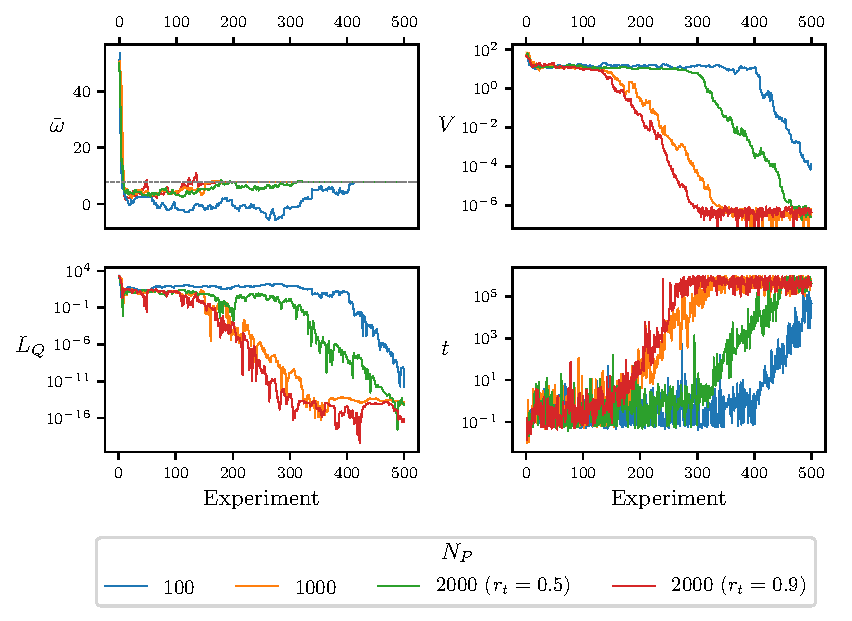
\includegraphics{algorithms/figures/params.pdf}
    \caption[Parameter learning with varying number of particles]{
        Parameter learning for the analyitcal \gls{likelihood} \cref{eqn:analytical_likleihood}
        for varying numbers of \glspl{particle} \gls{nprt}, for $\Ne=500$. 
        For $\Np=2000$, we show the resampler threshold set to $r=0.5$ and $r=0.9$. 
        \textbf{a,} the parameter estimate, i.e. $\bar{\omega}$, the mean of the posterior distribution after each experiment, 
        approaching $\omega_0=7.75$ (dashed line), where the prior is centred on $\omega=50 \pm 25$. 
        Decrease in \textbf{(b)} volume, $V$, \textbf{(c)} quadratic loss, $L_Q$, 
        and \textbf{(d)} evolution time, $t$, are shown against \gls{experiment} number.
        \figtableref
    }
    \label{fig:param_learning_vary_particles}
\end{figure}


\gls{qhl} is a parameter estimation algorithm, so here we introduce some methods to evaluate its performance, 
    which we can reference in later sections of this thesis. 
The most obvious meausre of the progression of parameter estimation is the error between the true parameterisation, 
    $\al_0$, and the approximation $\al_p = \mean \bk{ \Pr(\al) }$,
    which can be captured by a large family of loss functions. 
Among others, we use the \gls{ql}, which captures this error through the sum of the square difference between 
    each parameters' true and estimated values symetrically.
We can record the \gls{ql} at each \gls{experiment} of our training regime and hence track its over- or under-esimtation. 
The \gls{ql} is given by 
    \begin{equation}
        \label{eqn:quadratic_loss}
        L_{Q}(\al) = \left\| \al_0 - \al \right\|^2
    \end{equation}
    where $\al_0$ is the true parameterisation and $\al$ a hypothesis distribution.
\par 

\subsection{Volume}\label{sec:volume}
We also care about the range of parameters supported by $\Pr(\al)$ at each experiment: 
    the \gls{volume} of the \gls{particle} distribution can be seen as a proxy for our certainty
    that the approximation $\mean\bk{\Pr(\al)} $ is accurate. 
For example, for a single parameter $\omega$, our best knowledge of the parameter is $\mean\bk{ \Pr(\omega) }$, 
    and our belief in that approximation is the standard deviation of $\Pr(\omega)$; 
    we can think of \gls{volume} as an $n$-dimensional generalisation of this intuition \cite{qinfer-1_0, ferrie2014high}. 
\par 
In general, a confidence region, defined by its confidence level $\kappa$, is drawn by grouping \glspl{particle} 
    of \emph{high \gls{particle} density}, $\mathcal{P}$, such that $\sum\limits_{p \in \mathcal{P}} w_{p} \geq \kappa$.
We use the concept of \emph{minimum volume enclosing ellipsoid}
    to capture the confidence region \cite{ferrie2014high}, calculated as in \cite{todd2007khachiyan}, 
    which are characterised by their covariance matrix, $\Sigma$, which allows us to calculate the \gls{volume}, 
    \begin{equation}
        \label{eqn:volume}
        V(\Sigma) = \frac{ \pi^{| \al | / 2}}{ \Gamma(1 + \frac{| \al |}{2})} \det\bk{\Sigma^{-\frac{1}{2}}},
    \end{equation}
    where $\Gamma$ is the Gamma function, and $|\al|$ is the cardinality of the parameterisation. 
This quantity allows us to meaningfully compare distributions of different dimension, 
    but we must be cautious of drawing strong comparisons between models based on 
    their \gls{volume} alone, for instance because they may have started from vastly different prior distributions. 
\par 

Within \gls{smc}, we assume the credible region is simply the posterior distribution, 
    such that we can take $\Sigma = \textrm{cov}(\Pr(\al))$ after each experiment, 
    and hence track the uncertainty in our parameters across the training \glspl{experiment} \cite{Granade:2012kj}.
We use \gls{volume} as a measure of the learning procedure's progress: 
    slowly decreasing or static \gls{volume} indicates poor learning, possibly highlighting poor \gls{experiment} design, 
    while decreasing \gls{volume} indicates that the parameters' estimation is improving.
When the \gls{volume} has converged, e.g. the red model in \cref{fig:param_learning_vary_particles},
    the learning has saturated and there is little benefit to running further \glspl{experiment}. 

\section{Experiment design heuristic}\label{sec:heuristic}
A key consideration in \gls{qhl} is the choice of experimental controls implemented in attempt to learn from the system. 
The experimental controls required are dictated by the choice of  \gls{likelihood} function used within \gls{smc}, 
    though typically there are two primary controls we will focus on: 
    the evolution time, $t$, and the \emph{\gls{probe}} state evolved, $\ket{\psi}$. 
The design of \glspl{experiment} is handled by an \gls{edh}, 
    whose structure can be altered to suit the user's needs, with respect to the individual target system. 
Usually, the \gls{edh} attempts to exploit the information available, 
    adaptively accounting for some aspects of the inference process performed already. 
In some cases, however, there may be justification to employ a non-adaptive schedule, 
    for instance to force \gls{qhl} to train upon a full set of experimental data rather than a subset,
    as an adaptive method may advise.
We can categorise each \gls{edh} as either \emph{online} of \emph{offline},
    depending on whether it accounts for the current state of the inference procedure, i.e. the posterior.
The \gls{edh} is modular and can be replaced by any method that returns a valid set of experimental controls, 
    so we can consider numerous approaches, for instance those described in \cite{hincks2018hamiltonian, fiderer2020neural}.
\par 

\subsection{Particle guess heuristic}\label{sec:pgh}
The default \gls{edh} is the \gls{pgh} \cite{Wiebe:2014qhl}, 
    an online method which attempts to design the optimal evolution time based on the posterior at each experiment.
Note \gls{pgh} does not specify the \gls{probe}, so is coupled with a \gls{probe} selection routine to comprise 
    a complete \gls{edh}.
\par

The principle of \gls{pgh} is that the uncertainty of the posterior limits how well the \gls{hamiltonian} is currently 
    approximated, and therefore limits the evolution time for which the posterior can be expected to 
    reasonably mimic $\ho$\footnotemark.
\footnotetext{
    The reasoning behind limiting the evolution time according to the posterior distribution is 
    rooted in the effect of the \acrlong{le}, described in \cref{sec:iqle}.
}
For example, consider \cref{eqn:analytical_hamiltonian} with a single parameter with $\omega_0 = 10$,
    and current $\mean\bk{\Pr(\omega)} = 9, \std\bk{\Pr(\omega)} = 2$:
    we can expect that the approximation $\omega^{\prime} = \mean\bk{\Pr(\omega)}$ 
    is valid up to $t_{max} \approx \nicefrac{1}{\std\bk{\Pr(\omega)}}$. 
% TODO make a figure illustrating this point with some wide, medium and thin priors
It is sensible, then, to use $t \sim t_{max}$ for two reasons: 
    (i) smaller times are already well explained by the posterior, so offer little opportunity to learn;
    (ii) $t_{max}$ is at or near the threshold which \glspl{particle} sampled from the posterior can comfortably explain, 
        so it will expose the relative difference in \gls{likelihood} between the posterior's better and worse \glspl{particle}, 
        providing a capacity to learn. 
Informally, as the uncertainty in the posterior shrinks, \gls{pgh} selects larger times 
    to ensure the training is based on informative eperiments while 
    simultaneously increasing certainty about the paraemters. 
In the one-dimensional case, this logic can be used to find an optimal time heuristic, 
    where \gls{experiment} $k$ is assigned $t_k = \nicefrac{1.26}{\std\bk{\Pr(\omega)}}$ \cite{ferrie2013best}. 
\par
For a general multidimensional parameterisation, 
    rather than directly using the inverse of the standard deviation of $\pr{\al}$, 
    which relies on the expensive calculation of the covarinace matrix, 
    \gls{pgh} uses a proxy whereby two \glspl{particle} are sampled from $\pr{\al}$. 
The experimental evolution time for \gls{experiment} $k$ is then given by 
\begin{equation}
    \label{eqn:pgh_time}
    t_k = \frac{1}{\| \al_i - \al_j \|}, 
\end{equation}
    where $\al_i, \al_j$ are distinct \glspl{particle} sampled from $\mathcal{P}$ where 
    $\mathcal{P}$ is the set of \glspl{particle} under consideration by \gls{smc} after \gls{experiment} $k-1$, 
    which had been recently sampled from $\Pr\bk{\al}$. 
\par 


\subsection{Alternative experiment design heuristics}\label{sec:alt_heuristics}
The \gls{edh} can be specified to the requirements of the target system; 
    we test four examples of customised \glspl{edh} against four target \glspl{hamiltonian}.
Here the \gls{edh} must only design the evolution time for the experiment, 
    with \gls{probe} design discussed in the next section. 
The heuristics tested are:

\begin{easylist}
    \ListProperties(Numbers=r)
    & $\textrm{Random}(0, t_{max})$: Randomly chosen time up to some arbitrary maximum, we set $t_{max} = 1000$ (arbitrary units). 
        This approach is clearly subobtimal, since it does not account whatsoever for the knowledge of the training so far, 
        and demands the user choose a suitable $t_{max}$, which can not gauranteed to be meaningful. 
    & $t$ list: forcing the training to consider a set of times decided in advance.
        For instance, when only a small set of experimental measurements are available, it is sensible to train on all of them, perhaps repeatedly. 
        We test uniformly spaced times between 0 and $t_{max}$, and cycle through the list twice, 
            aiming first to broadly learn the region of highest likelihood for all times, and then to refine the approximation.
        Again this \gls{edh} fails to account for the performance of the trainer so far, so may use times either 
        far above or below the ability of the parameterisation. 
    & $(\nicefrac{9}{8})^k$: An early attempt to match the expected exponential decrease in \gls{volume} from the training, 
        was to set $t_k = (\nicefrac{9}{8})^k$ \cite{Granade:2012kj}.
        Note we increment $k$ after 10 \glspl{experiment} in the training regime, 
        rather than after each experiment, which would result in extremely high times which flood  \gls{cpu} memory.
    & \Gls{pgh}: as described in \cref{sec:pgh}. 
\end{easylist}

We demonstrate the influence of the \gls{edh} on the training procedure
    by testing models\footnotemark \ of various complexity amd dimension in \cref{fig:heuristics_test}.
\footnotetext{
    Note the models designed here are not intended to represent physically meaningful situations, 
    but merely to serve as examples of simulatable \glspl{hamiltonian}. 
}
In particular, we first test a simple 1-qubit model, \cref{eqn:qhl_test_model_1}; 
    followed by more complicated 1-qubit model, \cref{eqn:qhl_test_model_2};
    as well as randomly generated 5-qubit Ising, \cref{eqn:qhl_test_model_3}, and 4-qubit Heisenberg models, \cref{eqn:qhl_test_model_4}.
Each $\hi$ have randomly chosen parameters implicitly assigned to each term. 
\begin{subequations}\label{eqn:qhl_test_models}
    \begin{equation}
        \label{eqn:qhl_test_model_1}
        \h_1=\s^z_1
    \end{equation}
    \begin{equation}
        \label{eqn:qhl_test_model_2}
        \h_2 = \s^x_1 + \s^y_1 + \s^z_1
    \end{equation}
    \begin{equation}
        \label{eqn:qhl_test_model_3}
        \h_3 = \s^z_1\s^z_3 + \s^z_1\s^z_4 + \s^z_1\s^z_5 + \s^z_2\s^z_4 +\s^z_2\s^z_5 + \s^z_3+\s^z_4 + \s^z_3+\s^z_5
    \end{equation}
    \begin{equation}
        \label{eqn:qhl_test_model_4}
        \h_4 = \s^z_1\s^z_2 + \s^z_1\s^z_3 +\s^x_2\s^x_3 + \s^z_2\s^z_3 + \s^x_2\s^x_4 + \s^z_3\s^z_4
    \end{equation}
\end{subequations}

\begin{figure}
    \begin{center}
        % \QMLAfig{Nov_27/heuristic_comparisons.pdf}
        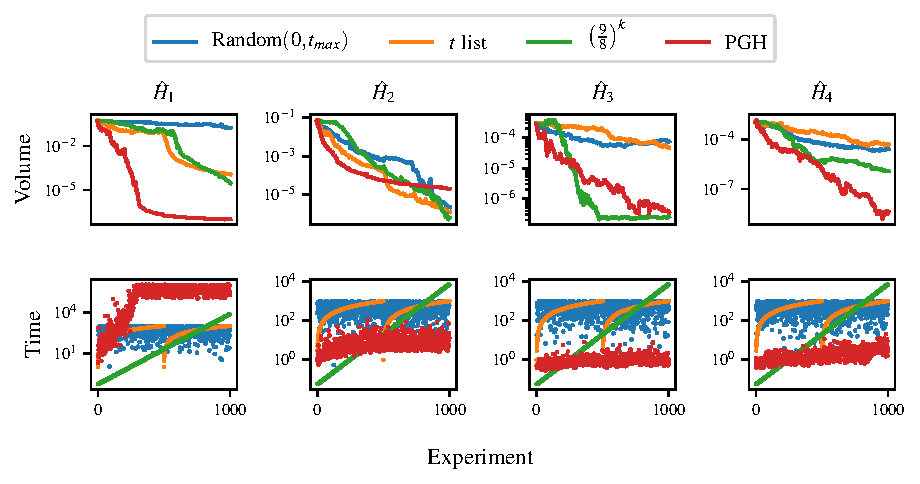
\includegraphics{algorithms/figures/heuristic_comparisons.pdf}
    \end{center}
    \caption[Effect on model training of the experiment design heuristic]{
        The \gls{volume} (top) and evolution times (bottom) of various models when trained through \gls{qhl} using different \glspl{edh}.
        We show models of various complexity and dimension, each trained using four heuristics, 
        outlined in the main text.
        \figtableref
    }
    \label{fig:heuristics_test}
\end{figure}

We show the performance of each of the listed \glspl{edh} in \cref{fig:heuristics_test}. 
The general trend reveals that, although some individual models benefit from bespoke \glspl{edh}, 
    the \gls{pgh} is generically applicable and usually facilitates a reasonable level of training, 
    without providing advantage to any model. 
We will have cause to use alternative \glspl{edh} in paricular circumstances, 
    but we adopt \gls{pgh} as the default \gls{edh} throughout this thesis, 
    unless otherwise stated.

\section{Probe selection}\label{sec:probes}

A final consideration about training \glspl{experiment} within \gls{qhl} is the choice of input \gls{probe} state, $\ket{\psi}$,
    which is evolved in the course of finding the \gls{likelihood} used during the Bayesian update. 
We can consider the choice of \gls{probe} as an output of the \gls{edh},  
    although previous work has usually not considered optimising the \gls{probe}, 
    instead usually setting $\ket{\psi} = \ket{+}^{\otimes n}$ for $n$ qubits \cite{wang2017experimental, ferrie2013best}.
In principle it is possible for the \gls{edh} to design a new \gls{probe} at each experiment, 
    although a more straightforward approach is to compose a set of probes offline, $\Psi = \{ \ket{\psi} \}$,
    of size $\Npsi = \absval{\Psi}$.
Then, a \gls{probe} is chosen at each \gls{experiment} from $\Psi$, 
    allowing for the same $\ket{\psi}$ to be used for multiple \glspl{experiment} within the training, e.g. by iterating over $\Psi$. 
$\Psi$ can be generated with respect to the individual learning problem as we will examine later, 
    but it is usually sufficient to use generic strategies which should work for all models;
    some straightforward examples are
    \begin{easylist}[enumerate]
        \ListProperties(Numbers=r)
        & $\ket{0} : \ \Psi = \{\ket{0}^{\otimes n}\}, \ \ \Npsi=1$;
        & $\ket{+} : \ \Psi = \{\ket{+}^{\otimes n}\}, \ \ \Npsi=1$;
        & $\ket{t} : \ \Psi$ is a random subset of probes generated by combining tomographic basis states, \ \ $\Npsi=40$;
        & $\ket{r} : \ \ket{\psi}$ are random, separable probes, \ \ $\Npsi=40$.
    \end{easylist}
\par 
We show the 1-qubit probes within $\Psi$ under each of these strategies on the Bloch sphere in \cref{fig:probes_used_bloch}.

\begin{figure}
    \begin{center}
        \subfloat{
            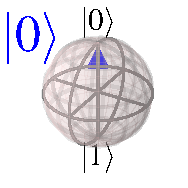
\includegraphics{algorithms/figures/zero_probes.pdf}
        }
        \qquad
        \subfloat{
            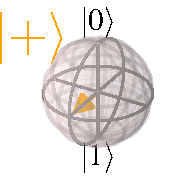
\includegraphics{algorithms/figures/plus_probes.pdf}
        }
        \qquad
        \subfloat{
            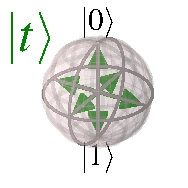
\includegraphics{algorithms/figures/tomographic_probes.pdf}
        }
        \qquad
        \subfloat{
            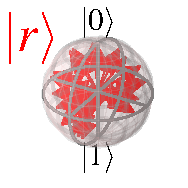
\includegraphics{algorithms/figures/random_probes.pdf}
        }
        \qquad
    \end{center}
    \caption[Probes used for tests]{
        1-qubit probes used for tests in \cref{fig:probes_test}.
    }
    \label{fig:probes_used_bloch}
\end{figure}

\begin{figure}
    \begin{center}
        % \QMLAfig{Nov_27/training_probes.pdf}
        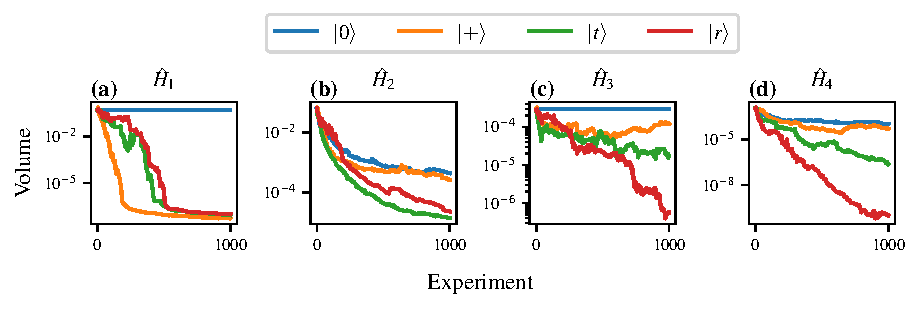
\includegraphics{algorithms/figures/training_probes.pdf}
    \end{center}
    \caption[Training with different probes]{
        The \gls{volume} of various models when trained through \gls{qhl} using different initial \gls{probe} sets. 
        We show models of various complexity and dimension, each trained using random probes, $\ket{r}$, 
        tomographic basis set probes, $\ket{t}$, as well as $\ket{0}$ and $\ket{+}$ probes. 
        In each case the probes are generated for arbitrary numbers of qubits; 
        for $\ket{0}, \ket{1}$, the number of probes generated is $N_{\psi}=1$, 
        and for $\ket{t}, \ket{r}$, $N_{\psi}=40$.
        \figtableref
    }
    \label{fig:probes_test}
\end{figure}

Recalling the set of models from \cref{eqn:qhl_test_models},
    we test each of these \gls{probe} construction strategies in \cref{fig:probes_test}. 
We can draw a number of useful observations from these simple tests: 
\begin{easylist}[itemize]
    & Training on an eigenstate 
        -- as in the case for $\hat{H}_1$ and $\hat{H}_3$ using $\ket{0}$ --  
        yields no information gain. 
        This is because all \glspl{particle} give \glspl{likelihood}  $l=1$, 
        so no weight update can occur, meaning the parameter distribution does not change when presented new evidence. 
    & Training on an even superposition of the model's eigenstates 
        -- e.g. $\ket{+}$ for $\hat{H}_1$ --  
        is maximally informative: 
        any deviations from the true parameterisation are registered most dramatically in this basis,
        providing the optimal training \gls{probe} for this case.     
    & These observations are reinforced by \cref{fig:probes_test}\textbf{c}, where a 5-qubit Ising model also 
        fails to learn from one of its eigenstates, $\ket{0}^{\otimes 5}$.
        Of note, however, is that $\ket{+}^{\otimes 5}$ is not the strongest \gls{probe} here: the much larger Hilbert space here 
        can not be scanned sufficiently using a single probe; 
        using a larger number of probes is more effective, even if those are randomly chosen. 
    & In general the tomographic and random \gls{probe} sets perform reliably, 
        even for complex models.
\end{easylist}

It is an open challenge to identify the optimal \gls{probe} for training any given model;
    the design of informative probes could be built into the \gls{edh} in principle,
    e.g. a set of \glspl{probe} could be generated of even superpositions of the candidate's eigenstates.
However, for model comparison purposes in general, 
    it is helpful to have a universal set of probes, $\Psi$, upon which all models are trained. 
The use of $\Psi$ minimises systematic bias towards particlar models, 
    which might arise from probes which server as favourable bases for a subset of models, 
    for example $\ket{+}$ in \cref{fig:probes_test}\textbf{a}. 
Careful consideration should be given to $N_{\psi}$ in the choice of the \gls{probe} generator, 
    since it is important to ensure probes robustly test the parameterisation across the entire Hilbert space.
It is also necessary that \gls{smc} has sufficient opportunity to learn within a given subspace before moving to the next, 
    so that slight deviations in $\Pr(\al)$ due to a single probe are not immediately reversed because a distant probe is immediately invoked. 
We can mitigate this concern by instructing the \gls{edh} to repeatedly select a \gls{probe} from $\Psi$ for a batch of successive \glspl{experiment}, 
    before moving to the next available probe. 
Unless otherwise stated, for the remainder of this thesis we will adopt the random \gls{probe} 
    generator as the defualt mechanism for selecting probes,
    iterating between probes after batches of 5 \glspl{experiment}.
